\documentclass{oci}
\usepackage[utf8]{inputenc}
\usepackage{lipsum}
\usepackage{tikz}
\usepackage{pgfplots}
\usetikzlibrary{shapes.misc}

\tikzset{cross/.style={cross out, draw=black, inner sep=0pt, outer sep=0pt},
%default radius will be 1pt.
cross/.default={1pt}}

\title{El juego del calendario}

\begin{document}
\begin{problemDescription}
  Alicia acaba de inventar un juego muy particular.
  Para poder jugarlo solo se necesita un lápiz y el calendario de un mes de 30 días.
  Las fechas de cada mes se numeran de 1 a 30, y el día de la semana correspondiente al inicio del mes 
  podrá variar según el mes del que se trate. 
  Por ejemplo, la siguiente imagen muestra el calendario de un mes que comienza un viernes.
  \begin{center}
    \scalebox{0.8}{
      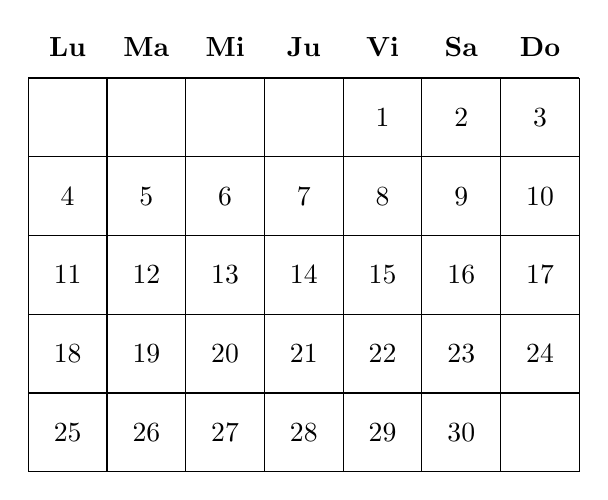
\begin{tikzpicture}
        \draw (0, 0) grid (7, 5);
        \def\weeks{5}
        \def\start{4}
        \foreach \d [count=\x from 0] in {Lu, Ma, Mi, Ju, Vi, Sa, Do}{
          \node at (\x + 0.5, \weeks + 0.4) {\textbf{\d}};
        };
        \foreach \i in {0, ..., 29}{
          \pgfmathtruncatemacro{\x}{Mod(\start + \i, 7)}
          \pgfmathtruncatemacro{\y}{(\start + \i) / 7}
          \pgfmathtruncatemacro{\d}{\i + 1}
          \node[fill=white] at (\x + 0.5, \weeks - \y - 0.5) {\d};
        }
      \end{tikzpicture}
    }
  \end{center}

  El juego inicia escogiendo una fecha inicial $x$, la que se considera como \emph{visitada} y debe ser tachada de inmediato.
  Posteriormente, se debe aplicar una regla que indica a qué fecha hay que moverse; es decir, cuál será la siguiente fecha a visitar. 
  La regla que hay que aplicar en cada paso depende del día de la semana en el que cae la fecha que se está visitando actualmente.
  El juego termina instantáneamente cuando se visita una fecha $y$ que ya había sido visitada antes.
  
  En algunos casos no será posible aplicar la regla correspondiente, por lo que no se podrá seguir visitando nuevas fechas. En esta situación, 
  consideraremos que el juego terminó en la última fecha visitada satisfactoriamente.
  
  % El juego termina cuando una regla indica que hay que moverse a un día que ya había sido tachado
  % o cuando no es posible aplicar una regla.
  
  Las reglas para cada día de la semana se detallan a continuación:
  \begin{itemize}
   \item[\bf Lunes] Avanzar de una en una por las fechas del calendario hasta encontrar una que no haya sido tachada, y moverse a dicha fecha.
    Si al avanzar buscando una fecha sin tachar se llega al final del mes, se debe \emph{dar la vuelta} y continuar avanzando desde el inicio del mes.
    Si no queda ninguna fecha sin tachar, la regla no puede aplicarse y el juego termina en el día actual.

    \item[\bf Martes] Moverse a la fecha que corresponde al \emph{reflejo} de la fecha actual.
    Es decir, si la fecha actual es $i$, la siguiente fecha a visitar será la $31 - i$.

    \item[\bf Miércoles] Si la fecha actual es par, moverse a la fecha anterior.
    Si la fecha actual es impar, moverse a la fecha siguiente.

    \item[\bf Jueves] Moverse a la fecha que está 10 posiciones adelante, dando la vuelta en caso de
    llegar al final del mes.

    \item[\bf Viernes] Si la fecha actual $i$ es par, moverse a la fecha $i/2$.
    En caso contrario, moverse a la fecha $3\times i + 1$.
    Si $3\times i + 1$ es mayor que 30, se debe restar 30 al resultado hasta que este sea menor o igual que 30.

    \item[\bf Sábado] Si la fecha actual es $i$, moverse a la fecha $2\times i$.
    Si $2\times i$ es mayor que 30, se debe restar 30 al resultado hasta que este sea menor o igual que 30.

    \item[\bf Domingo] Avanzar de dos en dos por las fechas del calendario hasta encontrar una que no haya sido tachada, y moverse a esta fecha.
    Dar la vuelta al mes en caso de ser necesario.
    Si no se puede avanzar a ninguna fecha sin tachar, la regla no puede aplicarse y el juego termina en el día actual.
  \end{itemize}

  Considera el calendario del ejemplo mostrado anteriormente donde el inicio del mes cae un viernes.
  Si escogemos como fecha inicial $x=16$, notamos que esta cae un sábado.
  La regla para el sábado dice que hay que moverse a la fecha $2\times 16 = 32$; como este valor es mayor que 30,
  restamos 30 una vez y nos movemos a la fecha 2.
  La fecha 2 cae un sábado nuevamente y por lo tanto la siguiente fecha a visitar es $2\times 2=4$.
  La fecha 4 cae un lunes. La regla del lunes dice que hay que encontrar la siguiente fecha no tachada, que corresponde al martes 5.
  La regla para el martes nos pide movernos al reflejo, que en este caso corresponde a la fecha $31 - 5 = 26$.
  La fecha 26 corresponde nuevamente a un martes y la regla nos pide movernos a la fecha $31 - 5 = 5$, que ya había
  sido visitada previamente y por lo tanto \textbf{el juego termina el martes 5}.
  La siguiente imagen muestra la secuencia de movimientos descritos anteriormente:

  \begin{center}
    \scalebox{0.8}{
      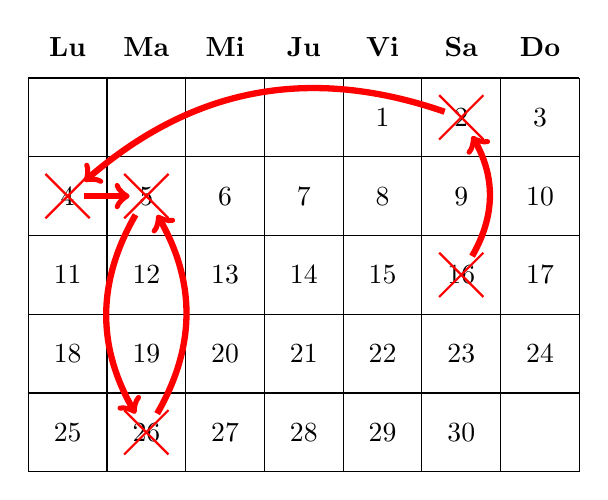
\begin{tikzpicture}
        \draw (0, 0) grid (7, 5);
        \def\weeks{5}
        \def\start{4}
        \foreach \d [count=\x from 0] in {Lu, Ma, Mi, Ju, Vi, Sa, Do}{
          \node at (\x + 0.5, \weeks + 0.4) {\textbf{\d}};
        };
        \foreach \i in {0, ..., 29}{
          \pgfmathtruncatemacro{\x}{Mod(\start + \i, 7)}
          \pgfmathtruncatemacro{\y}{(\start + \i) / 7}
          \pgfmathtruncatemacro{\d}{\i + 1}
          \node[fill=white] (\d) at (\x + 0.5, \weeks - \y - 0.5) {\d};
        }
        \node[cross, thick, red, minimum size=16] at (16) {};
        \node[cross, thick, red, minimum size=16] at (2) {};
        \node[cross, thick, red, minimum size=16] at (4) {};
        \node[cross, thick, red, minimum size=16] at (5) {};
        \node[cross, thick, red, minimum size=16] at (26) {};
        \draw[->,red, line width=0.8mm, bend right] (16) edge (2);
        \draw[->,red, line width=0.8mm, bend right] (2)  edge (4);
        \draw[->,red, line width=0.8mm]             (4)  edge (5);
        \draw[->,red, line width=0.8mm, bend right] (5)  edge (26);
        \draw[->,red, line width=0.8mm, bend right] (26) edge (5);
      \end{tikzpicture}
    }
  \end{center}

  Dado el día de la semana en el que inicia el mes y la fecha inicial $x$ con que comienza
  el juego, tu tarea es ayudar a Alicia a determinar en qué fecha del mes finaliza el juego.
\end{problemDescription}

\begin{inputDescription}
  La entrada contiene una línea con dos enteros: $d$ ($0 \leq d \leq 6$) y $x$ ($1 \leq x \leq 30$).
  El entero $d$ corresponde al día de la semana en el que comienza el mes.
  Si $d$ es $0$, el mes comienza un lunes; si $d$ es $1$, el mes comienza un martes; y así hasta el domingo.
  El entero $x$ indica la fecha inicial del juego.
\end{inputDescription}

\begin{outputDescription}
  La salida debe contener un único entero indicando la fecha en la que termina el juego.
\end{outputDescription}

\begin{scoreDescription}
  Este problema no contiene subtareas. Se entregará puntaje proporcional a la cantidad de casos
  de prueba correctos, siendo 100 el puntaje máximo.
  % \subtask{40}
  % Se probarán varios casos donde $d = 0$, es decir, el mes siempre comienza un lunes.
  % \subtask{60}
  % Se probarán varios casos sin restricciones adicionales.
\end{scoreDescription}

\begin{sampleDescription}
\sampleIO{sample-1}
\sampleIO{sample-2}
\end{sampleDescription}

\end{document}
